\documentclass[answers]{exam}
\usepackage{../../mypackages}
\usepackage{../../macros}

\SolutionEmphasis{\color{blue}}
\renewcommand{\solutiontitle}{\noindent}

\title{Interrogation N°2 - Peinture / Minéraux / Restauration}
\author{N. Bancel}
\date{Novembre 2024}

\begin{document}

\textbf{Collège Lycée Suger}
\hfill
\textbf{Physique-Chimie} \\

\textbf{Année 2024-2025 - 3ème trimestre}
\hfill
\textbf{1ères STD2A} \par

{\let\newpage\relax\maketitle}

\begin{center}
\textbf{\textcolor{red}{Durée : 45 minutes. La calculatrice n'est pas autorisée}} \\
\textbf{\textcolor{red}{Une réponse donnée sans justification sera considérée comme fausse.}} \\
Cette interrogation contient \numquestions\ questions, sur \numpages\ pages et est notée sur \numpoints\ points. 
\end{center}

\section{Partie 1 : La peinture}

\begin{questions}

  \question[4] Brièvement définir chacun des constituants de la peinture, et donner un exemple (reproduire sur votre copie et remplir le tableau)

  \begin{center}
    \begin{tabular}{|>{\bfseries}l|p{7cm}|p{4cm}|}
    \hline
    Constituant & Définition & Exemple \\
    \hline
    Liant &  &  \\
    \hline
    Diluant / Solvant &  &  \\
    \hline
    Pigment & &  \\
    \hline
    Charges &  &  \\
    \hline
    Additifs &  &  \\
    \hline
    \end{tabular}
    \end{center}

  

\begin{solution}


\subsection*{Constituants de la peinture}

\begin{center}
\begin{tabular}{|>{\bfseries}l|p{7cm}|p{4cm}|}
\hline
Constituant & Définition & Exemple \\
\hline
Liant & Le liant est utilisé pour fixer les pigments et permettre à la peinture d'adhérer à la surface sur laquelle elle est appliquée. & Résine acrylique \\
\hline
Diluant / Solvant & Le diluant, ou solvant, est utilisé pour ajuster la viscosité de la peinture et faciliter son application. & Eau (pour les peintures acryliques) \\
\hline
Pigment & Les pigments sont des substances colorantes qui donnent à la peinture sa couleur. & Oxyde de titane \\
\hline
Charges & Les charges sont des matériaux qui améliorent certaines propriétés de la peinture, comme sa texture ou son pouvoir couvrant. & Carbonate de calcium \\
\hline
Additifs & Les additifs sont utilisés pour modifier les propriétés de la peinture, telles que le temps de séchage ou la résistance aux intempéries. & Agents anti-UV \\
\hline
\end{tabular}
\end{center}


\end{solution}

\question[1] Que signifie une peinture "sans solvant" ?
  

\begin{solution}

\subsection*{Peinture "sans solvant"}

Une peinture "sans solvant" signifie une peinture qui ne contient pas de diluant utilisé pour ajuster sa viscosité. Les peintures sans solvant sont formulées pour minimiser l'émission de composés organiques volatils (COV) dans l'atmosphère. Elles sont souvent à base d'eau, ce qui les rend plus respectueuses de l'environnement et moins nocives pour la santé.

\end{solution}

\question[1] Expliquer la différence entre le séchage par évaporation et le séchage par siccavation.  
  

\begin{solution}

\subsection*{Différence entre séchage par évaporation et séchage par siccavation}

\begin{compactitem}
    \item \textbf{Séchage par évaporation} :
    \begin{compactitem}
        \item Le séchage par évaporation est un processus physique où le solvant de la peinture s'évapore.
        \item Ce type de séchage dépend de la température et de la ventilation.
        \item Aucune réaction chimique n'est impliquée; seul le solvant quitte le film de peinture.
    \end{compactitem}
    
    \item \textbf{Séchage par siccavation} :
    \begin{compactitem}
        \item Le séchage par siccavation est un processus chimique où la peinture durcit grâce à l'oxydation du liant.
        \item Ce processus implique une réaction chimique, généralement l’oxydation d’huiles ou de résines naturelles.
        \item Le séchage dépend de l'oxygène présent dans l'air, et non de l'évaporation.
    \end{compactitem}
\end{compactitem}

Ainsi, la principale différence réside dans le fait que le séchage par évaporation est un processus physique nécessitant l'évaporation du solvant, tandis que le séchage par siccavation est un processus chimique impliquant la durcissement du liant via l'oxydation.

\end{solution}

\question[2] Indiquer la différence entre le pigment et le colorant.

  \end{questions}



\begin{solution}

\subsection*{Différence entre pigment et colorant}

\begin{compactitem}
    \item \textbf{Pigment} : 
    \begin{compactitem}
        \item Les pigments sont des substances en poudre qui ne se dissolvent pas dans le milieu qu'ils colorent.
        \item Ils sont insolubles et restent en suspension dans un liant.
        \item Les pigments sont souvent utilisés pour leur capacité à fournir une couleur intense et durable.
    \end{compactitem}
    
    \item \textbf{Colorant} :
    \begin{compactitem}
        \item Les colorants sont des substances qui se dissolvent dans le milieu qu'elles colorent.
        \item Ils sont solubles, ce qui permet une dispersion uniforme de la couleur.
        \item Les colorants peuvent être utilisés pour teindre des liquides ou des matériaux où une solution homogène est requise.
    \end{compactitem}
\end{compactitem}

Ainsi, la distinction principale réside dans la solubilité : les pigments sont insolubles et restent en suspension, alors que les colorants sont solubles et se dissolvent dans le milieu.

\end{solution}

\section{Partie 2 : Les minéraux}

\begin{questions}

\question[2] Qu'est ce qu'un solide amorphe ?


\begin{solution}
Un solide amorphe est un type de solide qui, contrairement aux cristaux, ne présente pas de structure ordonnée à l'échelle microscopique. Dans un solide amorphe, les atomes ou molécules sont disposés de manière aléatoire, ce qui signifie qu'il n'y a pas de répétition régulière d'un motif sur de longues distances. Cette absence d'ordre cristallin donne aux solides amorphes des propriétés physiques distinctes, telles qu'une absence de points de fusion nets.

\subsection*{Conclusion}

Les solides amorphes sont courants dans la nature et dans les matériaux fabriqués par l'homme, tels que le verre, les plastiques, et certains types de gels. Leur structure irrégulière rend ces solides généralement moins rigides et plus malléables que les solides cristallins.
\end{solution}

\question[2] Quel est le principal composant du verre ? 


\begin{solution}
Le principal composant du verre est la silice, \ce{SiO2}.  

\subsection*{Conclusion}

La silice est un composé chimique formé de silicium et d'oxygène, qui constitue la majorité de la composition du verre. Sa structure amorphe, où les atomes ne sont pas arrangés de manière régulière, confère au verre ses propriétés uniques, telles que la transparence et la résistance aux intempéries.
\end{solution}

\question[1] Qu'est ce que la température de transition vitreuse ? On pourra s'aider d'un schéma pour justifier. 


\begin{solution}
La température de transition vitreuse, notée souvent \( T_g \), est une température caractéristique des matériaux amorphes, tels que le verre et certains polymères. Elle marque la transition de l'état de solide "rigide" à un état plus "caoutchouteux" ou visqueux. Cette transition ne correspond pas à un changement de phase net, comme une fusion, mais plutôt à un changement progressif des propriétés mécaniques et physiques du matériau lorsque sa température augmente.

\subsection*{Explication avec schéma}

\begin{center}
  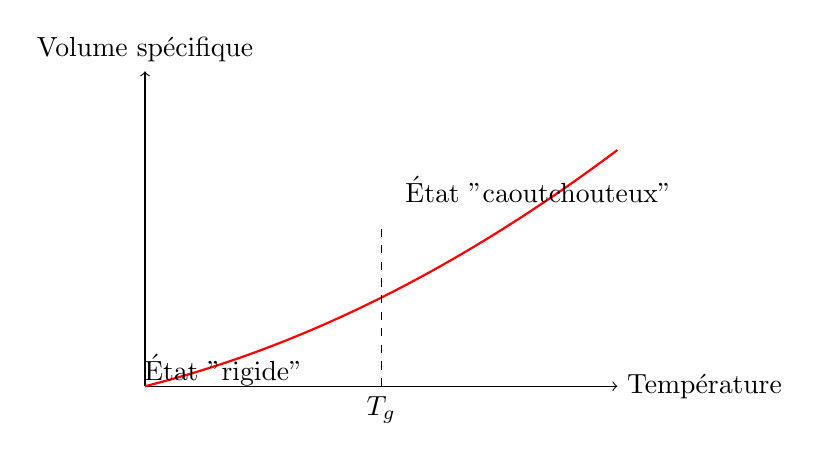
\begin{tikzpicture}
    % Axes
    \draw[->] (0,0) -- (6,0) node[anchor=west]{Température};
    \draw[->] (0,0) -- (0,4) node[anchor=south]{Volume spécifique};

    % Ligne de transition
    \draw[thick, red] (0,0) .. controls (2,0.5) and (4,1.5) .. (6,3);

    % Point de transition vitreuse
    \draw[dashed] (3,0) -- (3,2);

    % Labels
    \node at (3,-0.3) {\( T_g \)};
    \node at (5,2.5) {État "caoutchouteux"};
    \node at (1,0.2) {État "rigide"};

  \end{tikzpicture}
\end{center}

\begin{addmargin}[2em]{1em}
  \begin{compactitem}
      \item La courbe représente le changement du volume spécifique du matériau avec l'augmentation de la température. 
      \item En dessous de \( T_g \), le matériau est dans un état rigide.
      \item Au-dessus de \( T_g \), le matériau devient plus souple et visqueux.
  \end{compactitem}
\end{addmargin}

\subsection*{Conclusion}

La température de transition vitreuse est fondamentale pour déterminer les applications possibles des matériaux amorphes. Par exemple, pour un verre utilisé dans des applications architecturales, \( T_g \) doit être bien au-dessus des températures attendues dans cet environnement pour éviter toute déformation.
\end{solution}

\question[1] Ce qui distingue une céramique d'un verre est que la céramique a une structure majoritairement cristalline. Citer 2 propriétés physiques intéressantes de la céramique.

\end{questions}



\begin{solution}
Les céramiques, du fait de leur structure majoritairement cristalline, possèdent plusieurs propriétés physiques intéressantes. En voici deux :

\begin{compactitem}
    \item \textbf{Haute résistance mécanique :} Les céramiques sont généralement très dures et résistantes à la compression. Cette propriété en fait des matériaux idéaux pour des applications nécessitant une grande résistance à l'usure et à la déformation, comme les outils de coupe ou les revêtements de sol.

    \item \textbf{Stabilité thermique :} Les céramiques conservent leurs propriétés mécaniques à des températures élevées. Elles présentent une faible dilatation thermique et sont souvent utilisées dans des environnements sujet à des variations de température importantes, comme les éléments réfractaires dans les fourneaux.

\end{compactitem}

Ces propriétés rendent les céramiques précieuses dans des domaines tels que l'électronique, l'aérospatial, et la construction.
\end{solution}

\section{Partie 3 : La restauration}

\begin{questions}

\question[2] Quelle est la différence entre une méthode destructive et une méthode non destructive ? Donner un exemple de chaque.


\begin{solution}

\subsection*{Différence entre méthode destructive et méthode non destructive}

Lors de l'analyse ou de la restauration d'un objet, il existe deux types de méthodes utilisées : les méthodes destructives et les méthodes non destructives.

\begin{compactitem}
    \item \textbf{Méthode destructive :} 
        \begin{addmargin}[4em]{1em}
        Une méthode destructive implique l'altération ou la destruction partielle ou totale de l'objet analysé. Ces méthodes sont souvent utilisées lorsqu'une analyse précise et détaillée est nécessaire, par exemple, en chimie analytique pour déterminer la composition exacte d'un échantillon.\\
        \textit{Exemple :} L'analyse chimique par dissolution, où une partie de l'échantillon est dissoute pour en déterminer la composition.
        \end{addmargin}

    \item \textbf{Méthode non destructive :} 
        \begin{addmargin}[4em]{1em}
        Une méthode non destructive permet de préserver l'intégrité de l'objet testé ou analysé. Ces techniques sont employées lorsque l'objet doit être conservé intact après l'analyse.\\
        \textit{Exemple :} L'imagerie par rayons X, utilisée pour examiner l'intérieur d'un objet sans causer de dommages.
        \end{addmargin}
\end{compactitem}

\end{solution}

\question[2] Quel type d'information sur une oeuvre les méthodes vues en cours permettent-elles de déterminer ?


\begin{solution}

\subsection*{Informations déterminées par les méthodes d'analyse}

Les méthodes d'analyse vues en cours, qu'elles soient destructives ou non destructives, permettent de déterminer plusieurs types d'informations importantes sur une œuvre :

\begin{compactitem}
    \item \textbf{Composition chimique :} Ces méthodes permettent de découvrir les matériaux et les substances utilisés dans l'œuvre, par exemple, les pigments dans une peinture.
    \item \textbf{Structure interne :} Grâce à des techniques comme l'imagerie par rayons X, il est possible de visualiser les couches sous-jacentes ou la structure interne sans endommager l'œuvre.
    \item \textbf{État de conservation :} Elles peuvent évaluer l'état de dégradation des matériaux, ce qui est essentiel pour planifier une restauration efficace.
    \item \textbf{Techniques de fabrication :} Les analyses permettent aussi de comprendre les techniques et procédés utilisés par l'artiste, ce qui contribue à la valorisation historique de l'objet.
\end{compactitem}

Ces informations sont cruciales non seulement pour la préservation et la restauration des œuvres d'art, mais aussi pour enrichir notre compréhension historique et culturelle.

\end{solution}

\question[1] Expliquer brièvement la méthode de datation au carbone 14 


\begin{solution}

\subsection*{Méthode de datation au carbone 14}

La datation au carbone 14 est une méthode utilisée pour déterminer l'âge d'objets organiques jusqu'à environ \SI{50000}{ans}. Elle repose sur le principe de la décroissance radioactive du carbone 14, un isotope radioactif du carbone.

\begin{compactitem}
    \item \textbf{Principe :} Le carbone 14 se forme dans l'atmosphère et est absorbé par les organismes vivants. Lorsque ceux-ci meurent, ils cessent de l'absorber, et le carbone 14 commence à se désintégrer à un taux constant.
    
    \item \textbf{Formule :} La méthode utilise la formule :
    \[
    N(t) = N_0e^{-\lambda t}
    \]
    où 
    \begin{addmargin}[4em]{1em}
    \begin{compactitem}
        \item [$N(t)$]: représente la quantité de carbone 14 à un instant $t$
        \item [$N_0$]: représente la quantité initiale de carbone 14
        \item [$\lambda$]: est la constante de désintégration du carbone 14
        \item [$t$]: le temps écoulé depuis la mort de l'organisme
    \end{compactitem}
    \end{addmargin}
    
    \item \textbf{Conclusion :} En mesurant la quantité de carbone 14 restant dans l'échantillon et en utilisant la demi-vie connue du carbone 14 (\SI{5730}{ans}), il est possible de calculer l'âge de l'échantillon.
\end{compactitem}

La datation au carbone 14 est une technique précieuse en archéologie et paléontologie pour dater des restes biologiques anciens.

\end{solution}

\question[1] Donner les valeurs limites des longueurs d'onde du domaine visible.


\begin{solution}

\subsection*{Longueurs d'onde du domaine visible}

Le domaine visible du spectre électromagnétique correspond aux longueurs d'onde que l'œil humain peut percevoir. 

Les valeurs limites des longueurs d'onde du domaine visible sont environ :

\begin{compactitem}
    \item \textbf{Limite inférieure :} \SI{380}{\nano\meter} (violet)
    \item \textbf{Limite supérieure :} \SI{750}{\nano\meter} (rouge)
\end{compactitem}

Ainsi, le spectre visible s'étend grosso modo de \SI{380}{\nano\meter} à \SI{750}{\nano\meter}.

\end{solution}

\question[1] Les rayonnements infrarouges sont invisibles pour l'oeil humain. Citer un autre type de rayonnement invisible utilisé dans l'étude d'oeuvres d'art.

\end{questions}



\begin{solution}

\subsection*{Autre type de rayonnement invisible}

En plus des rayonnements infrarouges, un autre type de rayonnement invisible souvent utilisé dans l'étude des œuvres d'art est l'ultraviolet (UV). Le rayonnement UV permet de révéler des détails invisibles à l'œil nu, comme les retouches ou les couches de vernis. Il est souvent utilisé car il peut provoquer une fluorescence distinctive de certains matériaux, ce qui est utile pour l'analyse de la surface et de la composition des œuvres.

\end{solution}

\end{document}
